\section{Count-min sketch: range queries}

Show and analyze the application of count-min sketch to range queries $(i,j)$ for computing  $\sum^j_{k=i} F[k]$. Hint: reduce the latter query to the estimate of just $t \leq 2 \log n$ counters $c_1,c_2,...,c_t$. Note that in order to obtain a probability at most $\delta$ of error (i.e. that $\sum^t_{l=1}c_l > \sum^j_{k=i}F[k] + 2\varepsilon \log n ||F||$), it does not suffices to say that it is at most $\delta$ the probability of error of each counter $c_l$: while each counter is still the actual wanted value plus the residual as before, it is better to consider the sum $V$ of these $t$ wanted values and the sum $X$ of these residuals, and apply Markov’s inequality to $V$ and $X$ rather than on the individual counters.

\vspace{1cm}
\noindent
\textbf{Solution.} A range $[a,b]$ is a dyadic range if its length is a power of two ($l=2^y$), and begins at a multiple of its own length: $[j2^y+1, (j+1)2^y]$. For example, $[13,16]$ can be written as $[3\cdot 2^2+1,(3+1)\cdot 2^2]$. Any arbitrary range of size $s$ can be partitioned into $O(\log s)$ dyadic ranges \cite{Cormode11}, for example:
$$[18,38]=[18,18]\cup[19,20]\cup[21,24]\cup[25,32]\cup[33,36]\cup[37,38].$$

Let $n$ be the size of the implicit vector $F$ whose entries we want to approximate. The idea is to maintain a collection $C=\marray{T_0, T_1, \dots, T_{\log_2 n-1}}$ of $\log_2 n$ CM sketches, such that $T_y$ is responsible for the set of dyadic ranges of length $2^y$ $\forall y\in [0, \log_2 n-1]$. The operations on $C$ becomes:
\begin{itemize}
  \item \textbf{Update}, that is, given $i,v$, approximate $F[i] = F[i] + v$. Every sketch in $C$ is updated, since each point $1 \leq i \leq n$ is member of $\log_2 n$ dyadic ranges.
  \item \textbf{Range queries}, that is, given $l, r$, approximate $\sum_{i=l}^rF[i]$. The range $[l,r]$ is partitioned into at most $2\log_2 n$ dyadic ranges. For each partition of size $2^y$, a point query is made to the corresponding sketch $T_y$; the (estimated) result of the range query is the sum of the point queries. See Figure \ref{figure:dyadic-ranges}.
\end{itemize}

The time to compute the estimate or to make an update is $O(\log n\log\frac{1}{\delta})$. The space used is $O(\frac{1}{\varepsilon}\log n\log\frac{1}{\delta})$, because each sketch requires $O(\frac{e}{\varepsilon}\ln\frac{1}{\delta})$ space \cite{Cormode05}.

Let $F[l..r]=\sum_{i=l}^rF[i]$ be the answer to the range query and $\tilde{F}[l..r]$ the estimate. The guarantees are
\begin{itemize}
  \item $\tilde{F}[l..r] \geq F[l..r]$, and
  \item $\prob{\tilde{F}[l..r] > F[l..r]+2\varepsilon\log n\norm{F}} \leq \delta$.
\end{itemize}

\begin{proof}
  Let $I_{i,j,k}$ the indicator variable that is $1$ if $i \ne k \wedge h_j(i)=h_j(k)$ and $0$ otherwise. From the analysis of CM sketch, we know that
  $\E{I_{i,j,k}} \leq \frac{\varepsilon}{e}$,
  and
  $$\E{X_{i,j}} = \E{\sum_{k=1}^n I_{i,j,k}F[k]} \leq \frac{\varepsilon}{e}\norm{F}.$$
  A range query $\tilde{F}[l..r]$ is assembled by  $t \leq 2\log n$ point queries on dyadic intervals $[l_1,r_1], [l_2,r_2], \dots, [l_t,r_t]$. 
  The expectation of the additive error $X^j$ for any estimator (i.e. the $j$th row of any of the $t$ CM sketches queried) is
  \begin{equation}
    \E{X^j} = \E{\sum_{s=1}^tX_{i,j}}=\sum_{s=1}^t\E{X_{i,j}} \leq (2\log n) \frac{\varepsilon}{e}\norm{F}.
    \label{range-query-error-expect}
  \end{equation}
  Also observe that the $j$th estimation of $F[l..r]$ is
  \begin{equation}
    \tilde{F}^j[l..r]= \sum_{s=1}^t \tilde{F}^j[l_s..r_s] = \sum_{s=1}^t (F[l_s..r_s] + X_{i,j}) = F[l..r]+X^j.
    \label{range-query-f}
  \end{equation}
  Now, for the $j$th estimation we can compute
  \begin{align*}
    &\phantom{={}} \prob{\tilde{F}^j[l..r] > F[l..r]+2\varepsilon\log n\norm{F}} & \\
    &= \prob{X^j > 2\varepsilon\log n\norm{F}} & \text{because of \eqref{range-query-f}} \\
    &\leq \frac{\E{X^j}}{2\varepsilon\log n\norm{F}} & \text{by the Markov inequality} \\
    &\leq  \frac{2\varepsilon\log n\norm{F}}{e} \frac{1}{2\varepsilon\log n\norm{F}} & \text{because of \eqref{range-query-error-expect}} \\
    &= e^{-1}. &
  \end{align*}
  Since we have $\ln\frac{1}{\delta}$ independent hash functions $\prod_{j=1}^{\ln(1/\delta)}e^{-1}=e^{-\ln(1/\delta)}=\delta$.
\end{proof}

\begin{figure}[h]
  \centering
  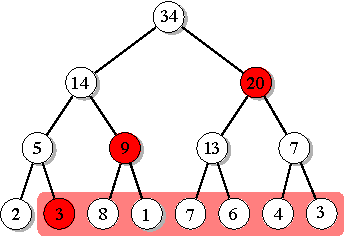
\includegraphics[width=0.55\linewidth]{images/dyadic-ranges}
  \caption{A hierarchy of dyadic ranges. The leaves are the ranges of length $2^0$, while the root corresponds to the single range of length $2^3$. Each level of the tree can be seen as a CM sketch table. To estimate $\sum_{k=2}^8F[k]$, the range $[2,8]$ is decomposed into dyadic ranges $[2,2], [3,4], [5,8]$. Each node contains the sum of the values stored in its children. Red nodes are queried and their sum is returned. Adapted from \cite{Cormode11}.}
    \label{figure:dyadic-ranges}
\end{figure}
